{ %section2_5
	\subsection{Measuring the runtime of parallel programs}
	\par\textbf{Time measuring tools.} Measuring the runtime of a program in C is not a difficult problem, however, in parallel programming, a number of specific difficulties arise in performing this operation. Not all functions suitable for measuring the running time of a sequential program are suitable for measuring the running time of a multithreaded program.
	\par For example, if you use the \texttt{ctime} or \texttt{localtime} functions in a single-threaded program to measure the operating time of a section of code, they will successfully cope with the task. However, after parallelizing this part of the code, it is possible that hard-to-identify problems arise with incorrect time measurement, because both of these functions have an internal static variable, which, when trying to change it simultaneously by several threads, can take an unpredictable value.
	\par In order to solve the described problem, some C-compilers (for example, gcc) implemented thread-safe, re-entrant versions of these functions: \texttt{ctime\textunderscore r} and \texttt{localtime\textunderscore r}. Unfortunately, these functions are not available in all compilers. For example, in the Visual Studio compiler, a similar problem was solved using functions with different names and APIs: \texttt{GetTickCount, GetLocalTime, GetSystemTime}. For completeness, we list some other gcc functions that also allow you to measure time: time, getrusage, gmtime, gettimeofday.
	\par Another standard C-function clock also cannot be used to measure the execution time of multithreaded programs. However, the reason for this is not the lack of reenterability, but the features of the way this function calculates the elapsed time: clock returns the number of processor ticks that were executed when the program was running in total with all its threads. Obviously, this amount remains almost unchanged when the program executes with a different number of threads ("almost'', since the overhead costs of creating, deleting and managing threads are proposed to be considered insignificant in order to simplify the presentation).
	\par As a result, it turned out that a satisfactory \textit{cross-platform} solution for thread-safe time measurement with high accuracy (up to microseconds) by means of pure C language does not exist yet. However, the problem can be solved using third-party libraries, choosing those that have an implementation on the target platforms.
	\par The OpenMP system, which is implemented in the vast majority of modern compilers for all modern operating systems, stands out among such libraries. OpenMP has two functions for measuring time: omp\textunderscore get\textunderscore wtime and omp\textunderscore get\textunderscore wtick, which can be used in C-programs, if you include the omp.h header file and specify the necessary key during compilation (for example, in gcc this is the key "{}-fopenmp").
	\par\textbf{Time measurement error.} Another interesting point in measuring the running time of a parallel program is the method by which the researcher excludes various random errors from measurements that inevitably arise during an experiment in a running operating system, which can start the update or optimization process without notifying the user. The generally accepted is the way in which the researcher conducts not one, but immediately N experiments with a parallel program, without changing the initial data. It turns out N time measurements, which in the general case will be different due to various random factors affecting the experiment. Further, one of the following methods is most often used:
	\begin{enumerate}
		\item\textit{The calculation of the confidence interval:} consider all N measurements is calculated confidence interval, e.g., using Student's method.
		\item\textit{Search for the minimum measurement:} among N measurements, the smallest is chosen and it is used as the final result.
	\end{enumerate}
	\par The first method gives the correct result only if the measurement errors are distributed according to the normal law. This is most often the case, therefore, the application of the method is justified and allows you to get additional information about the possible use of the tested program in living conditions of a running OS.
	\par The second method does not impose requirements on the form of the law of distribution of measurement errors, and this compares favorably with the previous one. In addition, for large N, the choice of the minimum metering will make it possible to exclude from the experiment all the background influences of the operating system and to obtain as an result an accurate measurement of the operating time of the program under ideal conditions.
	\par\textbf{Practical example.} Let us compare by example the methods described above to get rid of the error of experimental time measurements. We will measure the OpenMP overhead for creating and deleting threads as follows:
	\begin{figure}[H]
		\lstinputlisting{OpenMPExampleTimeMeasurement.cpp}
	\end{figure}
	In line 3, we instruct OpenMP that when entering the parallel area located further in the program, i threads are created. If you do not give this indication, OpenMP will create the number of threads by the number of calculators available in the system (cores or logical processors). In line 4, we start the parallel program area, OpenMP creates i threads. In line 5, we give instructions to execute the following simple instruction in only one thread (the rest of the threads will not do any work. This is necessary so that only the costs of creating / deleting threads fall in the measured time of work, and all other costs would be lost against their background. The parallel area ends in line 6. OpenMP deletes the i number of  threads from the memory. A more detailed description of the OpenMP commands used can be found in section~\ref{OpenMP:section}~\textit{''OpenMP Technology''} of this book.
	\par Experiments with this program were conducted on a computer with an Intel Core i5 processor (4 logical processors) with 8 gigabytes of RAM in the Debian Wheezy operating system. Empirically, it was revealed that the operating system used on an accessible hardware platform cannot create more than 381 threads in the OpenMP program (this explains the value in line 1). A total of $N = 100$ experiments were carried out, the results of which were processed by each of the two described methods. The results are shown in the Figure~\ref{OpenMPExpensesOnCreatingThreads:image}.
	\begin{figure}[H]
		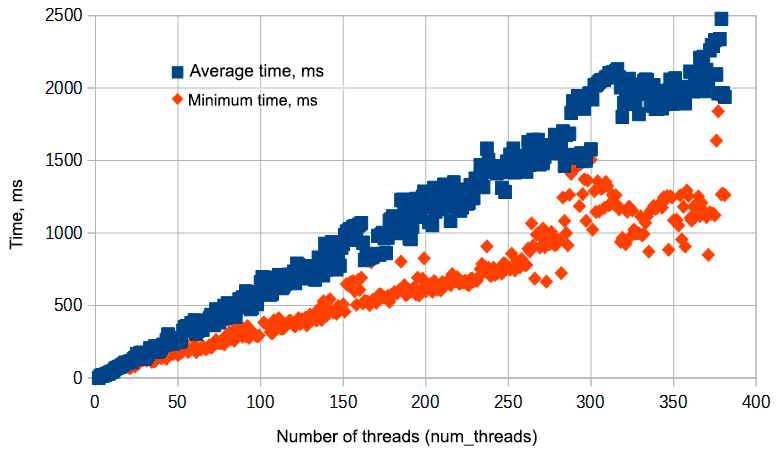
\includegraphics[width=1\linewidth]{OpenMPExpensesOnCreatingThreads}
		\caption{\textit{OpenMP overhead measurement results for thread creation and deletion}}
		\label{OpenMPExpensesOnCreatingThreads:image}
	\end{figure} 
	\par The measured value $(T2 - T1)$ in milliseconds is plotted along the ordinate axis, and the values of variable i, which indicate the number of created flows, are plotted on the abscissa axis. The upper graph, consisting of blue squares, shows the average value $(T2 - T1)$ for the 100 experiments performed. The confidence interval is not shown, as it would clutter the graph without adding informativeness, but the width of the confidence interval with a confidence level of 90 \% approximately corresponds to the vertical spread of the squares of the upper graph for neighboring values of i.
	\par The lower graph, consisting of rhombs, represents the minimum of 100 measurements $(T2 - T1)$ for the values of i indicated on the x-axis. We see that even a large number of experiments was not enough for the lower graph to have a smooth continuous structure without noticeable fluctuations.

}